After examining the preference-based consumer theory, we have concluded that if a continuously differentiable demand function $x(\mathbf{p},w)$ is generated by rational preferences, this demand function must have
certain properties (see Thm.\ref{thm:properties_walrasian_demand}) and have a symmetric and negative semidefinite substitution matrix $S(\mathbf{p},w)$. In this section, we would examine the reverse:
if a demand function $x(\mathbf{p},w)$ has these properties, can it be rationalized by some preferences?

\subsection{Recover Preferences from Demand Functions}\label{chp2:sec4:ssec1}
The recovering $\succsim$ from $x(\mathbf{p},w)$ will be done in 2 steps:
\begin{enumerate}
    \item[-] \textbf{Step 1}: recover $e(\mathbf{p},u)$ from $x(\mathbf{p},w)$
    \item[-] \textbf{Step 2}: recover $\succsim$ from $e(\mathbf{p},u)$  
\end{enumerate}

\subsubsection*{Recover $e(\mathbf{p},u)$ from $x(\mathbf{p},w)$}
The first step is to recover $e(\mathbf{p},u)$ given a Walrasian demand function $x(\mathbf{p},w)$ that has the assumed properties: satisfies Walras' law, homogeneous of degree 0(see Thm.\ref{thm:properties_walrasian_demand}).
And, demand is assumed to be single-valued.

The recovering of $e(\mathbf{p},u)$ relies on the duality property $h(\mathbf{p},u)=x(\mathbf{p},e(\mathbf{p},u))$ and the proposition $h(\mathbf{p},u)=\nabla_{\mathbf{p}}e(\mathbf{p},u)$, combine these two, get:
$$
    \frac{\partial e(\mathbf{p})}{\partial p_i}=x_i(\mathbf{p},e(\mathbf{p})),\forall i=1,\cdots,L
$$
or, in a familiar form of expression
$$
\nabla_{\mathbf{p}}e(\mathbf{p})=x(\mathbf{p},e(\mathbf{p}))
$$

For this system of differential equations to have a solution, we must have $e(\mathbf{p})$ to be \textbf{twice continuously differentiable}, i.e., $e(\mathbf{p})$'s Hessian matrix is \myhl[blue]{\textbf{symmetric}}. Do the twice differentiation of $e(\mathbf{p})$:
\begin{align*}
    \mathrm{D}^2_{\mathbf{p}}e(\mathbf{p}) &= \mathrm{D}_{\mathbf{p}}x(\mathbf{p},e(\mathbf{p})) +\mathrm{D}_w x(\mathbf{p},e(\mathbf{p}))\cdot x(\mathbf{p},e(\mathbf{p}))^T\\
    & = S(\mathbf{p},e(\mathbf{p}))
\end{align*}
we actually get the Slutsky matrix again. Now we can conclude

\begin{enumerate}
    \item[-] $\nabla_{\mathbf{p}}e(\mathbf{p})=x(\mathbf{p},e(\mathbf{p}))$ has a solution $\Leftrightarrow$ the Slutsky matrix $S(\mathbf{p},w)$ being \textbf{symmetric}
    \begin{enumerate}
        \item[-] $\Rightarrow$: proved by the above equation, which requires the Slutsky matrix be the Hessian matrix of $e(\mathbf{p})$, which aligns with Thm.\ref{thm:prop_hick_pricederive}
        \item[-] $\Leftarrow$: by Frobenius' theorem (see \hyperref[sssec:frobenius_theorem]{below} for details), the symmetry of $\nabla_{\mathbf{p}}$ at all points of its domain is equivalent to the existence of a solution 
    \end{enumerate}
    \item[-] the solution $e(\mathbf{p},u)$ has the properties of an expenditure function (Thm.\ref{thm:properties_expenditure_func}) $\Leftrightarrow$ the Slutsky matrix $S(\mathbf{p},w)$ being \textbf{negative semidefinite}
\end{enumerate}

Together, we have
\begin{proposition}{conditions of $S(\mathbf{p},w)$ to recover $e(\mathbf{p},u)$}{slutskycondition_recover}
    $S(\mathbf{p},w)$ being \myhl[blue]{\textbf{symmetric}} and \myhl[blue]{\textbf{negative semidefinite}} is the necessary and sufficient condition to recover $e(\mathbf{p},u)$
\end{proposition}

Prop.\ref{prop:slutskycondition_recover} is always true, and it can be linked to the discussion of WARP in the following way:
\begin{enumerate}
    \item[$L=2$] when there are only 2 goods, the Slutsky matrix is automatically symmetric, hence as long as the demand function $x(p_1,p_2,w)$ satisfies WARP (negative semidefiniteness guaranteed), $e(\mathbf{p},u)$ will be recovered:
    
    \begin{enumerate}
        \item[-] step 1: normalize $p_2=1$, pick an arbitrary price-wealth point $(p_1^0,1,w^0)$ and assign utility value $u^0$ to 
        \item[-] step 2: solve the differential equation 
        $$
        \frac{\mathrm{d}e(p_1)}{\mathrm{p_1}}=x_1(p_1,e(p_1))
        $$
        where $e(p_1)=e(p_1,1,u^0)$, $x_1(p_1,w)=x_1(p_1,1,w)$, with the initial condition $e(p_1^0)=w^0$
    \end{enumerate}
    Fig.\ref{fig:recover_exp_from_wal} illustrates the essence of this procedure intuitively: for any $(p_1,w)$, the demand function at the point $x_1(p_1,w)$ is the slope of some expenditure function, and for any given initial condition $(p_1^0,w^0)$, there will be an expenditure curve starts at it.
    \item[$L>2$] when there are more than 2 goods, WARP does not guarantee the symmetry of the Slutsky matrix, hence, symmetry condition must also be satisfied for the recovery of $e(\mathbf{p},u)$
\end{enumerate} 

\begin{figure}[ht]
    \centering
    \caption{Recover $e(\mathbf{p},u)$ from $x(\mathbf{p},w)$}
    \label{fig:recover_exp_from_wal}
    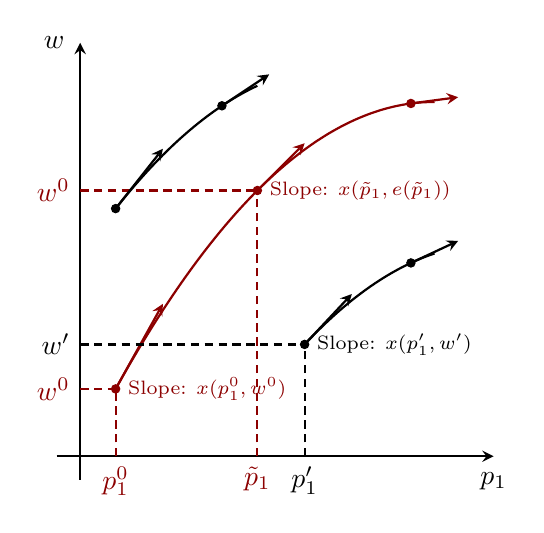
\begin{tikzpicture}[scale=1.5]
        % basics
        \draw [-stealth,color=black,thick] (-0.2,0) -- (3.5,0) node[below=2pt] {$p_1$};
        \draw [-stealth,color=black,thick] (0,-0.2) -- (0,3.5) node[left=2pt] {$w$};
        
        % correct e(p,u)
        \draw[domain=0.3:3, smooth, thick, red!55!black, variable=\x] plot ({\x}, {-1/3*(\x-3)^2+3});
        %% tangent 1
        \draw [-stealth,color=red!55!black,thick] (0.3,0.57) -- (0.7,1.29);
        \filldraw[red!55!black] (0.3,0.57) circle (1pt) node[right=1pt] {\scriptsize Slope: $x(p_1^0,w^0)$}; % initial bundle
        \draw[densely dashed,thick,red!55!black] (0.3,0) node[below] {$p_1^0$} --  (0.3,0.57);
        \draw[densely dashed,thick,red!55!black] (0,0.57) node[left] {$w^0$} -- (0.3,0.57);
        %% tangent 2
        \draw [-stealth,color=red!55!black,thick] (1.5,2.25) -- (1.9,2.65);
        \filldraw[red!55!black] (1.5,2.25) circle (1pt) node[right=1pt] {\scriptsize Slope: $x(\tilde{p}_1,e(\tilde{p}_1))$};
        \draw[densely dashed,thick,red!55!black] (1.5,0)  node[below] {$\tilde{p}_1$} -- (1.5,2.25);
        \draw[densely dashed,thick,red!55!black] (0,2.25) node[left] {$w^0$} -- (1.5,2.25);
        %% tangent 3
        \draw [-stealth,color=red!55!black,thick] (2.8,2.9867) -- (3.2,3.04);
        \filldraw[red!55!black] (2.8,2.9867) circle (1pt);
        
        % alternate 1
        \draw[domain=1.9:3, smooth, thick, black, variable=\x] plot ({\x}, {-1/3*(\x-3.5)^2+1.8});
        %% tangent a1
        \draw [-stealth,color=black,thick] (1.9,0.9467) -- (2.3,1.37337);
        \filldraw[black] (1.9,0.9467) circle (1pt) node[right=1pt] {\scriptsize Slope: $x(p'_1,w')$}; % initial bundle
        \draw[densely dashed,thick,black] (1.9,0) node[below] {$p'_1$} --  (1.9,0.9467);
        \draw[densely dashed,thick,black] (0,0.9467) node[left] {$w'$} -- (1.9,0.9467);
        %% tangent a2
        \draw [-stealth,color=black,thick] (2.8,1.6367) -- (3.2,1.82337);
        \filldraw[black] (2.8,1.6367) circle (1pt);
        
        % alternate 2
        \draw[domain=0.3:1.5, smooth, thick, black, variable=\x] plot ({\x}, {-1/3*(\x-2.2)^2+3.3});
        %% tangent b1
        \draw [-stealth,color=black,thick] (0.3,2.0967) -- (0.7,2.6033);
        \filldraw[black] (0.3,2.0967) circle (1pt);
        %% tangent b2
        \draw [-stealth,color=black,thick] (1.2,2.967) -- (1.6,3.233);
        \filldraw[black] (1.2,2.967) circle (1pt);
        
    \end{tikzpicture}
\end{figure}

\subsubsection*{Recover $\succsim$ from $e(\mathbf{p},u)$}
The second step is to recover $\succsim$ given an expenditure function $e(\mathbf{p},u)$ that has the assumed properties: continuous, strictly increasing in $u$, non-decreasing, homogeneous of degree 1, and concave in $\mathbf{p}$ (see Thm.\ref{thm:properties_expenditure_func}).
Since demand is single-valued, $e(\mathbf{p},u)$ is also differentiable.

Here, let $V_u\subset \mathbb{R}^L$  be an at-least-as-good-as set for each utility level $u$ s.t. $e(\mathbf{p},u)$ is the minimal expenditure required for a bundle in $V_u$ at price $\mathbf{p}\gg  0$, i.e. 
$$
e(\mathbf{p},u)=\min_{\mathbf{x}\geq 0}\mathbf{p}\cdot \mathbf{x}\ \text{ s.t. }\mathbf{x}\in V_u
$$

Intuitively, the set $V_u = \left\{ \mathbf{x} \in\mathbb{R}^L_+\mid \mathbf{p}\cdot \mathbf{x}\geq e(\mathbf{p},u),\forall \mathbf{p}\gg 0 \right\}$ satisfies the requirement, that is 
\begin{proposition}{At-least-as-good-as set $V_u$}{atleastasgoodasset_exp}
    For $e(\mathbf{p},u)$ that is strictly increasing in $u$, continuous, non-decreasing, homogeneous of degree 1, concave and differentiable in $\mathbf{p}$, then $\forall u$, $e(\mathbf{p},u)$ is the expenditure function associated with the at-least-as-good-as set
    $$
    V_u = \left\{ \mathbf{x}\in\mathbb{R}^L_+\mid \mathbf{p}\cdot\mathbf{x}\geq e(\mathbf{p},u),\forall \mathbf{p}\gg 0 \right\}
    $$
    i.e. $e(\mathbf{p},u)=\min\left\{ \mathbf{p}\cdot \mathbf{x}\mid \mathbf{x}\in V_u \right\},\forall \mathbf{p}\gg 0$.
\end{proposition}

\textbf{Proof}: Immediately by definitions, $e(\mathbf{p},u)\leq \min\left\{\mathbf{p}\cdot\mathbf{x}\mid \mathbf{x}\in V_n\right\}$. Next, prove $e(\mathbf{p},u)\geq \min\left\{\mathbf{p}\cdot\mathbf{x}\mid \mathbf{x}\in V_n\right\}$: since $e(\mathbf{p},u)$ is concave in $\mathbf{p}$, we have
$$
e(\mathbf{p}',u)\leq e(\mathbf{p},u)+\nabla_{\mathbf{p}}e(\mathbf{p},u)\cdot(\mathbf{p}'-\mathbf{p}),\forall \mathbf{p},\mathbf{p}'
$$
since $e(\mathbf{p},u)$ is homogeneous of degree 1, by Euler's formula, $e(\mathbf{p},u)=\mathbf{p}\cdot\nabla_{\mathbf{p}}e(\mathbf{p},u)$, hence $e(\mathbf{p}',u)\leq \mathbf{p}'\cdot \nabla_{\mathbf{p}}e(\mathbf{p},u),\forall \mathbf{p}'$, plus the fact that $\nabla_{\mathbf{p}(\mathbf{p},u)}\geq 0$, gives that $\nabla_{\mathbf{p}(\mathbf{p},u)}\in V_u$.
By the definition of the at-least-as-good-as set $V_u$, we have $\min\left\{\mathbf{p}\cdot\mathbf{x}\mid \mathbf{x}\in V_u\right\}\leq \mathbf{p}\cdot \nabla_{\mathbf{p}(\mathbf{p},u)}=e(\mathbf{p},u)$. The proof is finished.

With Prop.\ref{prop:atleastasgoodasset_exp}, we can find a set of $V_u$ for each level of $u$, and since $\partial e(\mathbf{p},u)/\partial u>0$, we have $u'>u\Rightarrow V_{u'}\subset V_u$. Each $V_u$ is closed, convex, and bounded below, hence these at-least-as-good-as sets can define a 
preference $\succsim$ (represented by utility levels $u$) that has $e(\mathbf{p},u)$ as its expenditure function (see Fig.\ref{fig:recover_pref_from_exp}).

\begin{figure}[ht]
    \centering
    \caption{Recover $\succsim$ from $e(\mathbf{p},u)$}
    \label{fig:recover_pref_from_exp}
    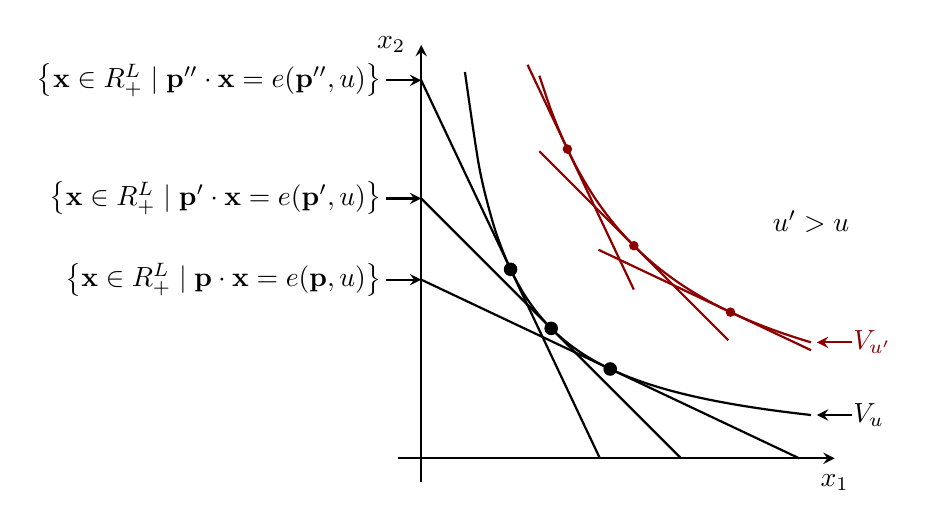
\begin{tikzpicture}[scale=1.5]
        % basics
        \draw [-stealth,color=black,thick] (-0.2,0) -- (3.5,0) node[below=2pt] {$x_1$};
        \draw [-stealth,color=black,thick] (0,-0.2) -- (0,3.5) node[left=2pt] {$x_2$};
        
        % utility and budget lines
        \draw[domain=0.37:3.3, smooth, thick, black, variable=\x] plot ({\x}, {1.1^2/\x}); % utility
        
        \draw[domain=1:3.3, smooth, thick, red!55!black, variable=\x] plot ({\x}, {1.8^2/\x}); % utility'
        
        \draw[domain=0:(4*1.1^2)/3.2, black, thick, variable=\x] plot ({\x}, {3.2-(3.2^2/(4*1.1^2))*\x}); % budget 1
        \draw[domain=0:2.2,black, thick, variable=\x] plot ({\x}, {2.2-\x}); % budget 2
        \draw[domain=0:3.2, black, thick, variable=\x] plot ({\x}, {((4*1.1^2)/3.2)-((4*1.1^2)/3.2^2)*\x}); % budget 3
        
        \draw[domain=0.9:1.8, red!55!black, thick, variable=\x] plot ({\x}, {5.23636-(3.2^2/(4*1.1^2))*\x}); % budget 1'
        \draw[domain=1:2.6,red!55!black, thick, variable=\x] plot ({\x}, {3.6-\x}); % budget 2'
        \draw[domain=1.5:3.3, red!55!black, thick, variable=\x] plot ({\x}, {2.475-((4*1.1^2)/3.2^2)*\x}); % budget 3'
        
        
        
        % bundles
        \filldraw[black] (0.75625,1.1^2/0.75625) circle (1.5pt); % bundle 1
        \filldraw[black] (1.1,1.1) circle (1.5pt); %  bundle 2
        \filldraw[black] (1.1^2/0.75625,0.75625) circle (1.5pt); % bundle 3
         % bundles
        \filldraw[red!55!black] (1.2375,1.8^2/1.2375) circle (1pt); % bundle 1'
        \filldraw[red!55!black] (1.8,1.8) circle (1pt); %  bundle 2'
        \filldraw[red!55!black] (1.8^2/1.2375,1.2375) circle (1pt); % bundle 3'
        
        %% utility
        \draw[stealth-,thick] (3.35,1.1^2/3.3) -- node[right=3pt] {$V_u$} (3.65,1.1^2/3.3);
        \draw[stealth-,thick,red!55!black] (3.35,1.8^2/3.3) -- node[right=3pt] {$V_{u'}$} (3.65,1.8^2/3.3);
        
        % texts and notes
        %% budget change
        \draw[-stealth,thick,black] (-0.3,3.2) -- node[left=4pt] {$\left\{\mathbf{x}\in\mathbb{R}^L_+\mid \mathbf{p}''\cdot\mathbf{x}=e(\mathbf{p}'',u) \right\}$} (0,3.2);
        \draw[-stealth,thick,black] (-0.3,2.2) -- node[left=4pt] {$\left\{\mathbf{x}\in\mathbb{R}^L_+\mid \mathbf{p}'\cdot\mathbf{x}=e(\mathbf{p}',u) \right\}$} (0,2.2);
        \draw[-stealth,thick,black] (-0.3,1.5125) -- node[left=4pt] {$\left\{\mathbf{x}\in\mathbb{R}^L_+\mid \mathbf{p}\cdot\mathbf{x}=e(\mathbf{p},u) \right\}$} (0,1.5125);
        
        \node at (3.3,2) {$u'>u$};
        
    \end{tikzpicture}
\end{figure}

This conclusion can be extended to the case that the underlying preferences of $e(\mathbf{p},u)$ is \textbf{non-convex}. A non-convex $\succsim$ will generate a non-convex 
at-least-as-good-as set, as shown in Fig.\ref{fig:recover_pref_from_exp_nonconvex}.

\begin{figure}[ht]
    \centering
    \caption{Recover non-convex $\succsim$ from $e(\mathbf{p},u)$}
    \label{fig:recover_pref_from_exp_nonconvex}
    \begin{tikzpicture}[scale=1.5]
        % basics
        \draw [-stealth,color=black,thick] (-0.2,0) -- (3.5,0) node[below=2pt] {$x_1$};
        \draw [-stealth,color=black,thick] (0,-0.2) -- (0,3.5) node[left=2pt] {$x_2$};
        
        \draw [thick,red!55!black,tangent=0.9] (0.37,3.3) .. controls (0.5,2.2) and (0.6,1.5) .. (0.8,1.5);
        \draw [black, thick, use tangent] (-1,0) -- (2,0);
        
        \draw [thick,red!55!black,tangent=0.1] (1.5,0.8) .. controls (1.5,0.6) and (2.2,0.5) .. (3.3,0.37);
        \draw [black, thick, use tangent] (-2,0) -- (1,0);
        
        %non-convex part
        \draw [thick,dashed,red!55!black] (0.8,1.5).. controls (1.4,1.4).. (1.5,0.8);
        \draw[domain=0.2:2.05,red!55!black, thick, variable=\x] plot ({\x}, {2.25-\x});
        
        % notes
        %%% actual
        \draw[stealth-,dashed, thick,red!55!black] (1.36,1.36) -- node[right=5pt,yshift=10pt,align=left] {Boundary of \textbf{actual} \\ at-least-as-good-as set} (1.7,1.7);
         %%% Slutsky
        \draw[-stealth,thick,black] (1.125-0.4,1.125-0.4) -- node[left=5pt,yshift=-10pt] {Boundary of $V_u$} (1.12,1.12);
        %%% price-utility
        \draw[stealth-,thick,black] (2.05,0.2) -- node[right=5pt] {\scriptsize $\left\{\mathbf{x}\in\mathbb{R}^L_+\mid \mathbf{p}^*\cdot\mathbf{x}=e(\mathbf{p}^*,u^*)\right\}$} (2.4,0.2);
    \end{tikzpicture}
\end{figure}

For this non-convex at-least-as-good-as set, we can always find its convex hull (the solid line) that also generates the
expenditure function $e(\mathbf{p}),u)$. 
Here we have the correspondence between the differentiability of $e(\mathbf{p},u)$ and the , for a specific price-utility pair $(\mathbf{p}^*,u^*)$, there would be more than one expenditure minimizers, and at this price-utility pair $(\mathbf{p}^*,u^*)$,
 the generated $e(\mathbf{p},u)$ would \textbf{NOT} be differentiable. This can be summarized as:
$$
e(\mathbf{p},u) \text{ is differentiable}\Rightarrow \succsim \text{ is convex}
$$

With the two steps, $\succsim$ can be recovered from demand function $x(\mathbf{p},w)$ through expenditure function $e(\mathbf{p},u)$. This problem, especially the problem of recovering $e(\mathbf{p},u)$ from $x(\mathbf{p},u)$, which involves the differential equation $h(\mathbf{p},u)=\nabla_{\mathbf{p}}e(\mathbf{p},u)$, is the \textbf{integrability} problem.

\subsubsection*{Discussion on integrability}\label{sssec:integrability}

\subsubsection*{Frobenius' theorem}\label{sssec:frobenius_theorem}
The Forbenius's theorem is one of the fundamental theorems in differential topology. It is the foundation for the disucssion of the integrability problem, which I think it's worth spending some time understanding the basics. The discussion below is by no means thorough or rigorous\footnote{For more math, check \cite{sternberg1999lectures}, \cite{warner1983foundations}, \cite{mccleary2013geometry}}, but my own interpretation of this topic.

\begin{definition}{Basic definitions of differntial geometry}{def}
    \begin{enumerate}
        \item[1] \textbf{smooth differentiable manifold} $M$ is a collection of \textbf{open} sets $U_{\alpha}\subset M$ and a collection of homeomorphisms $\varphi_{\alpha}:U_{\alpha}\rightarrow\mathbb{R}^N$ that satisfies
        \begin{enumerate}
            \item[-] $\bigcup_{\alpha}U_{\alpha}=M$ {(\color{red!55!black}$U_{\alpha}$\textit{ are the coordinate neighborhoods})}
            \item[-] when $U_{\alpha}\cap U_{\beta}\neq \varnothing$, the mapping $\varphi_{\alpha}\circ \varphi_{\beta}^{-1}:\varphi_{\beta}(U_{\alpha}\cap U_{\beta})\rightarrow \varphi_{\alpha}(U_{\alpha}\cap U_{\beta})$ is $C^{\infty}$ {\color{red!55!black}($M$ has a countable base)}
        \end{enumerate}
        \item[2] \textbf{coordinates}: define the $k-$th coordinate projection by $r^k\left(x^1,\cdots,x^N\right)=x^k$, then the coordinates on $M$ is 
        $$
        x^k = r^k\circ \varphi_{\alpha}: U_{\alpha}\rightarrow \mathbb{R}
        $$
        if $x\in U_{\alpha}$, $x$ is uniquely determined by its coordinates $\left(x^1(x),\cdots,x^m(x)\right)$
        \item[3] \textbf{tangent vectors} for a curve $\gamma:(-a,a)\rightarrow M$, its tangent vector $X$ maps a smooth function $f:M\rightarrow \mathbb{R}$ to its \underline{\textbf{directional derivative} $X(f)$} \sidenotes{$\leftarrow$ derivative of $f$ in the direction $X$}. At a point $x\in M$, the tangent vector is $$ X(f)_x\in \mathbb{R} $$ and it follows the rules of derivations (for smooth $f,g$)
        \begin{align*}
            X(fg)_x&=X(f)_xg(x)+f(x)X(g)_x & (aX+bY)(f)=aX(f)+bY(f)
        \end{align*} 
        denote the collection of tangent vectors at $x$ as $\mathrm{T}_x(M)$
        \item[4] \textbf{vector field}: for every $x\in M$, and the coordinates $x^k = r^k\circ \varphi$, the vector field is defined as
        $$
        \frac{\partial}{\partial x^k}(f)_x = \left.\frac{\partial (f\circ \varphi^{-1})}{\partial r^k}\right\vert_{\varphi(x)},\ k=1,\cdots,m
        $$
        and these tangent vectors $\left\{\frac{\partial}{\partial x^k}\right\}_{k=1}^m$ froms the basis for $\mathrm{T}_x(M)$, that is 
        $$
        X = \sum^m_{k=1}X^k\frac{\partial}{\partial x^k},\ \forall X\in\mathrm{T}_x(M)
        $$
    \end{enumerate}
\end{definition}